\chapter{State Machines}\label{state-machines}

This chapter defines language elements to define clocked state
machines. These state machines have a similar modeling power as
Statecharts (Harel 1987) and have the important feature that at one
clock tick, there is only one assignment to every variable (for example,
it is an error if state machines are executed in parallel and they
assign to the same variable at the same clock tick; such errors are
detected during translation). Furthermore, it is possible to activate
and deactivate clocked equations and blocks at a clock tick. An
efficient implementation will only evaluate the equations and blocks
that are active at the current clock tick. With other Modelica language
elements, this important feature cannot be defined.

The semantics of the state machines defined in this chapter is
inspired by mode automata and is basically the one from Lucid Synchrone
3.0 (Pouzet 2006). Note, safety critical control software in aircrafts
is often defined with such kind of state machines. The following
properties are different to Lucid Synchrone 3.0:
\begin{itemize}
\item
  Lucid Synchrone has two kinds of transitions: \emph{strong} and
  \emph{weak} transitions. Strong transitions are executed before the
  actions of a state are evaluated and weak transitions are executed
  after the actions of a state are evaluated. This can lead to
  surprising behavior, because the actions of a state are skipped if it
  is activated by a weak transition and exited by a true strong
  transition.

  For this reason, the state machines in this chapter use \emph{immediate}
  (= the same as \emph{strong}) and \emph{delayed} transitions. Delayed
  transitions are \emph{immediate} transitions where the condition is
  automatically delayed with an implicit \lstinline!previous!.
\item
  Parallel state machines can be explicitly synchronized with a
  language element (similarly as parallel branches in Sequential
  Function Charts). This often occurring operation can also be defined
  in Statecharts or in Lucid Synchrone state machines but only
  indirectly with appropriate conditions on transitions.
\item
  Modelica blocks can be used as states. They might contain
  clocked or clocked discretized continuous-time equations (in the
  latter case, the equations are integrated between the previous and the
  next clock tick, if the corresponding state is active).
\end{itemize}

\section{Transitions}\label{transitions}

Any Modelica block instance without continuous-time equations or
algorithms can potentially be a state of a state machine. A cluster of
instances which are coupled by \lstinline!transition! statements makes a
state machine. All parts of a state machine must have the same clock.
All transitions leaving one state must have different priorities. One
and only one instance in each state machine must be marked as initial by
appearing in an \lstinline!initialState! statement. The following special
kinds of connect-statements are used to define transitions between
states and to define the initial state:
\begin{longtable}[]{|p{4cm}|p{10cm}|}
\hline \endhead
\multicolumn{2}{|p{12cm}|}{\tablehead{Statements to define a state machine}}\\ \hline
\begin{tabular}{@{}p{4cm}@{}}
\lstinline!transition!(from, to,\\
condition,\\
immediate, reset,\\
synchronize, priority)
\end{tabular}
&
Arguments \lstinline!from! and \lstinline!to! are block instances and \lstinline!condition! is a
\lstinline!Boolean! argument. The optional arguments \lstinline!immediate!, \lstinline!reset!, and
\lstinline!synchronize! are of type \lstinline!Boolean!, have parametric variability and a
default of \lstinline!true!, \lstinline!true!, \lstinline!false! respectively. The optional
argument \lstinline!priority! is of type \lstinline!Integer!, has parametric variability and
a default of 1.

This operator defines a transition from instance \lstinline!from! to instance
\lstinline!to!. The \lstinline!from! and \lstinline!to! instances become states of a state
machine. The transition fires when \lstinline!condition = true! if
\lstinline!immediate = true! (this is called an \firstuse{immediate transition})
or \lstinline!previous(condition)! when \lstinline!immediate = false! (this is
called a \firstuse{delayed transition}). Argument \lstinline!priority! defines the
priority of firing when several transitions could fire. In this case the
transition with the smallest value of \lstinline!priority! fires. It is required
that $\textrm{priority}\ge 1$ and that for all transitions from the same state, the
priorities are different. If \lstinline!reset = true!, the states of the
target state are reinitialized, i.e.\ state machines are restarted in
initial state and state variables are reset to their start values. If
synchronize=true, any transition is disabled until all state machines of
the from-state have reached final states, i.e.\ states without outgoing
transitions. For the precise details about firing a transition, see
\cref{state-machine-semantics}.\\ \hline
\lstinline!initialState(state)! & Argument \lstinline!state! is the block instance
that is defined to be the initial state of a state machine. At the first
clock tick of the state machine, this state becomes active.\\ \hline
\end{longtable}

The transition-, and initialState-equations may only be used in
equations and may not be used inside if-equations with non-parametric
condition, or in when-equations.

It is possible to query the status of the state machine by using the
following operators:
\begin{longtable}[]{|p{4cm}|p{10cm}|}
\hline \endhead
\lstinline!activeState(state)!&
Argument \lstinline!state! is a block instance. The operator returns
\lstinline!true!, if this instance is a state of a state machine and this
state is active at the actual clock tick. If it is not active, the
operator returns \lstinline!false!.

It is an error if the instance is not a state of a state machine.\\ \hline
\lstinline!ticksInState()! & Returns the number of ticks of the clock of the state machine
for which the currently active state has maintained its active state without interruption,
i.e.\ without local or hierarchical transitions from this state.
In the case of a self-transition to the currently active state or to an active enclosing state,
the number is reset to one.
This function can only be used in state machines.\\ \hline
\lstinline!timeInState()! & Returns the time duration as \lstinline!Real! in {[}s{]}
for which the currently active state has maintained its active state without interruption,
i.e.\ without local or hierarchical transitions from this state.
In the case of a self-transition to the currently active state or to an active enclosing state,
the time is reset to zero.
This function can only be used in state machines.\\ \hline
\end{longtable}

\begin{example}
If there is a transition with \lstinline!immediate=false! from
state \lstinline!A1! to \lstinline!A2! and the condition is \lstinline!ticksInState() >= 5!, and \lstinline!A1! became
active at 10ms, and the clock period is 1ms, then \lstinline!A1! will be active at
10ms, 11ms, 12ms, 13ms, 14ms, and will be not active at 15 ms.
\begin{lstlisting}[language=modelica]
  block State end State;
  State A0;
  State A1; // Becomes active at 10ms
  State A2;
equation
  initialState(A0);
  transition(A0, A1, sample(time,Clock(1,1000)) > 0.0095);
  transition(A1, A2, ticksInState() >= 5, immediate=false);
\end{lstlisting}
\end{example}

\section{State Machine Graphics}\label{state-machine-graphics}

\begin{nonnormative}
\Cref{fig:state-machine-layout} shows the recommended layout of a state machine.

The recommended color is \{95, 95, 95\} for states and for transition text, and \{175,175,175\} for transition lines.
\end{nonnormative}

\begin{figure}[H]
  \begin{center}
    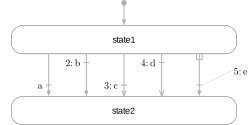
\includegraphics{statemachine}
  \end{center}
  % Avoid placing non-normative content in the caption.
  \caption{Recommended layout of a simple state machine.  For the 5 transitions, the settings are as follows, from left to right: \lstinline!immediate! = true, false, true, false, true; \lstinline!reset! = true, true, false, false, true; \lstinline!synchronize! = false, false, false, false, true; \lstinline!priority! = 1, 2, 3, 4, 5.}
  \label{fig:state-machine-layout}
\end{figure}

The annotation for graphics of \lstinline!transition! has the following
structure: \lstinline!annotation(Line($\ldots$), Text($\ldots$))!; and for
\lstinline!initialState()!: \emph{graphical-primitives}\lstinline!(Line($\ldots$))!; with \lstinline!Line!
and \lstinline!Text! annotations defined in \cref{annotations}.

\begin{example}
\begin{lstlisting}[language=modelica]
transition(state2, state1, x < 10, immediate=true, reset=true, synchronize=false, priority=1)
  annotation (
    Line(
      points={{-40,-16},{-36,-4},{-32,8},{-40,26},{-40,32},{-46,50}},
      color={175,175,175},
      thickness=0.25,
      smooth=Smooth.Bezier),
    Text(
      string="%condition",
      extent={{4,-4},{4,-10}},
      fontSize=10,
      textStyle={TextStyle.Bold},
      textColor={95,95,95},
      horizontalAlignment=TextAlignment.Left),
);
\end{lstlisting}
\end{example}

The Text annotation representing the transition condition can use the
notation \%condition to refer to the condition expression.

The extent of the Text is interpreted relative to either the first point
of the Line, in the case of immediate=false, or the last point
(immediate=true).

In addition to the line defined by the points of the Line annotation, a
perpendicular line is used to represent the transition. This line is
closer to the first point if immediate=false otherwise closer to the
last point.

If the condition text is somewhat distant from the perpendicular line, a
dimmed straight line joins the transition text and the perpendicular
line.  (See the rightmost transition above.)

If \lstinline!reset=true!, a filled arrow head is used otherwise an open arrow head.
For \lstinline!synchronize=true!, an inverse ``fork'' symbol is used in the
beginning of the arrow.  (See the rightmost transition above.)

The value of the \lstinline!priority! attribute is prefixing the condition text
followed by a colon if \lstinline!priority! \textgreater{} 1.

The \lstinline!initialState! line has a filled arrow head and a bullet at the
opposite end of the initial state (as shown above).

\section{State Machine Semantics}\label{state-machine-semantics}

For the purpose of defining the semantics of state machines, assume that
the data of all transitions are stored in an array of records:
\begin{lstlisting}[language=modelica]
record Transition
  Integer from;
  Integer to;
  Boolean immediate = true;
  Boolean reset = true;
  Boolean synchronize = false;
  Integer priority = 1;
end Transition;
\end{lstlisting}

The transitions are sorted with lowest priority number last in the
array; and the priorities must be unique for each value of \lstinline!from!. The
states are enumerated from 1 and up. The transition conditions are
stored in a separate array \lstinline!c[:]! since they are time varying.

The semantics model is a discrete-time system with inputs \{\lstinline!c[:]!,
\lstinline!active!, \lstinline!reset!\} with \lstinline!t! being an array corresponding to the inputs to the
transition operator, outputs \{\lstinline!activeState!, \lstinline!activeReset!,
\lstinline!activeResetStates[:]!\} and states \{\lstinline!nextState!, \lstinline!nextReset!,
\lstinline!nextResetStates[:]!\}. For a top level state machine, active is
always true. For sub-state machines, active is true only when the parent
state is active. For a top level state machine, reset is true at the
first activation only. For sub-state machine, reset is propagated from
the state machines higher up.

\subsection{State Activation}\label{state-activation}

The state update starts from \lstinline!nextState!, i.e., what has been determined to be the next state at the previous time.
\lstinline!selectedState! takes into account if a reset of the state machine is to be done.

\begin{lstlisting}[language=modelica]
output Integer selectedState = if reset then 1 else previous(nextState);
\end{lstlisting}
The integer fired is calculated as the index of the transition to be
fired by checking that \lstinline!selectedState! is the from-state and the condition
is true for an immediate transition or previous(condition) is true for a
delayed transition. The max function returns the index of the transition
with highest priority or 0.

\begin{lstlisting}[language=modelica]
Integer fired =
  max(
    if (if t[i].from == selectedState
        then (if t[i].immediate then c[i] else previous(c[i]))
        else false)
      then i
      else 0
    for i in 1:size(t,1));
\end{lstlisting}
The start value of c is false. This definition would require that the
previous value is recorded for all transitions conditions. Below is
described an equivalent semantics which just require to record the value
of one integer variable delayed.

The integer immediate is calculated as the index of the immediate
transition to potentially be fired by checking that \lstinline!selectedState! is the
from-state and the condition is true. The max function returns the index
of the transition with true condition and highest priority or 0.

\begin{lstlisting}[language=modelica]
Integer immediate =
  max(
    if (if t[i].immediate and t[i].from == selectedState
        then c[i]
        else false)
      then i
      else 0
    for i in 1:size(t,1));
\end{lstlisting}

In a similar way, the \lstinline!Integer delayed! is calculated as the index for a
potentially delayed transition, i.e.\ a transition taking place at the
next clock tick. In this case the from-state needs to be equal to
\lstinline!nextState!:
\begin{lstlisting}[language=modelica]
Integer delayed =
  max(
    if (if not t[i].immediate and t[i].from == nextState
        then c[i]
        else false)
      then i
      else 0
    for i in 1:size(t,1));
\end{lstlisting}

The transition to be fired is determined as follows, taking into account
that a delayed transition might have higher priority than an immediate:
\begin{lstlisting}[language=modelica]
Integer fired = max(previous(delayed), immediate);
\end{lstlisting}
\lstinline!nextState! is set to the found transitions to-state:
\begin{lstlisting}[language=modelica]
Integer nextState =
  if active then
    (if fired > 0
		  then t[fired].to
		  else selectedState)
	else
    previous(nextState);
\end{lstlisting}
In order to define synchronize transitions, each state machine must
determine which are the final states, i.e.\ states without
from-transitions and to determine if the state machine is in a final
state currently:
\begin{lstlisting}[language=modelica]
Boolean finalStates[nStates] = {
  max(if  t[j].from == i then 1 else 0 for j in 1:size(t,1)) == 0
  for i in 1:nStates};
Boolean stateMachineInFinalState = finalStates[activeState];
\end{lstlisting}
To enable a synchronize transition, all the stateMachineInFinalState
conditions of all state machines within the meta state must be true. An
example is given below in the semantic example model.

\subsection{Reset Handling}\label{reset-handling}

A state can be reset for two reasons:
\begin{itemize}
\item
  The whole state machine has been reset from its context.\\
  In this case, all states must be reset, and the initial state becomes
  active.
\item
  A reset transition has been fired.\\
  Then, its target state is reset, but not other states.
\end{itemize}

The first reset mechanism is handled by the activeResetStates and
nextResetStates vectors.

The state machine reset flag is propagated and maintained to each state
individually:
\begin{lstlisting}[language=modelica]
output Boolean activeResetStates[nStates] = {if reset then true else previous(nextResetStates[i]) for i in 1:nStates};
\end{lstlisting}
until a state is eventually executed, then its corresponding reset
condition is set to false:
\begin{lstlisting}[language=modelica]
Boolean nextResetStates[nStates] =
  if active then
    {if activeState == i then false else activeResetStates[i] for i in 1:nStates}
  else
    previous(nextResetStates)
\end{lstlisting}
The second reset mechanism is implemented with the selectedReset~and
nextReset~variables. If no reset transition is fired, the nextReset is
set to false for the next cycle.

\subsection{Activation handling}\label{activation-handling}

The execution of a sub-state machine has to be suspended when its
enclosing state is not active. This activation flag is given as a
\lstinline!Boolean! input \lstinline!active!. When this flag is true, the sub-state machine
maintains its previous state, by guarding the equations of the state
variables \lstinline!nextState!, \lstinline!nextReset! and \lstinline!nextResetStates!.

\subsection{Semantics Summary}\label{semantics-summary}

The entire semantics model is given below:
\begin{lstlisting}[language=modelica]
model StateMachineSemantics "Semantics of state machines"
  parameter Integer nStates;
  parameter Transition t[:] "Array of transition data sorted in priority";
  input
  Boolean c[size(t,1)] "Transition conditions sorted in priority";
  input Boolean active "true if the state machine is active";
  input Boolean reset "true when the state
machine should be reset";
  Integer selectedState = if reset then 1 else previous(nextState);
  Boolean selectedReset = if reset then true else previous(nextReset);
  // For strong (immediate) and weak (delayed) transitions
  Integer immediate = max(if (if t[i].immediate and t[i].from == selectedState
    then c[i] else false) then i else 0 for i in 1:size(t,1));
  Integer delayed = max(if  (if not t[i].immediate and t[i].from == nextState
    then c[i] else false) then i else 0 for i in 1:size(t,1));
  Integer fired = max(previous(delayed), immediate);
  output Integer activeState = if reset then 1 elseif fired > 0 then t[fired].to else selectedState;
  output Boolean activeReset = if reset then true elseif fired > 0 then t[fired].reset else selectedReset;

  // Update states
  Integer nextState = if active then activeState else previous(nextState);
  Boolean nextReset = if active then false else previous(nextReset);
  // Delayed resetting of individual states
  output Boolean activeResetStates[nStates] = {if reset then true else
    previous(nextResetStates[i]) for i in 1:nStates};
  Boolean nextResetStates[nStates] = if active then {if activeState == i then false
    else activeResetStates[i] for i in 1:nStates} else previous(nextResetStates);
  Boolean finalStates[nStates] = {max(if  t[j].from == i then 1 else 0 for j in 1:size(t,1))== 0 for i in 1:nStates};
  Boolean stateMachineInFinalState = finalStates[activeState];
end StateMachineSemantics;
\end{lstlisting}
\subsection{Merging Variable Definitions}\label{merging-variable-definitions}

\begin{nonnormative}
When a state class uses an \lstinline!outer output! declaration,
the equations have access to the corresponding variable declared
\lstinline!inner!. Special rules are then needed to maintain the single
assignment rule since multiple definitions of such outer variables in
different mutually exclusive states needs to be merged.
\end{nonnormative}

In each state, the outer output variables are solved for and for each
such variable a single definition is formed:
\begin{lstlisting}[language=modelica,escapechar=!]
v := if activeState(state!\textsubscript{1}!) then expre!\textsubscript{1}! elseif activeState(state!\textsubscript{2}!) then expre!\textsubscript{2}! elseif ... else last(v)
\end{lstlisting}

\lstinline!last! is special internal semantic operator returning its
input. It is just used to mark for the sorting that the incidence of its
argument should be ignored. A start value must be given to the variable
if not assigned in the initial state.

A new assignment equation is formed which might be merged on higher
levels in nested state machines.

\subsection{Merging Connections to Multiple Outputs}\label{merging-connections-to-multiple-outputs}

\begin{nonnormative}
Since instances of blocks can be used as states of a state
machine it is natural to extend the connection semantics of Modelica to
allow several outputs to be connected to one input.
\end{nonnormative}

It is possible to connect several outputs to an input if all the outputs
come from states of the same state machine. In such cases, we get the
following constraint equations:
\begin{lstlisting}[language=modelica,escapechar=!]
u!\textsubscript{1}! = u!\textsubscript{2}! = ... = y!\textsubscript{1}! = y!\textsubscript{2}! = ...
\end{lstlisting}
with u\textsubscript{i} inputs and y\textsubscript{i} outputs. The
semantics is defined as follows. Introduce a variable v representing the
signal flow and rewrite the equation above as a set of equations for
u\textsubscript{i} and a set of assignment equations for v:
\begin{lstlisting}[language=modelica,escapechar=!]
v := if activeState(state!\textsubscript{1}!) then y!\textsubscript{1}! else last(v);
v := if activeState(state!\textsubscript{2}!) then y!\textsubscript{2}! else last(v);
...
u!\textsubscript{1}! = v
u!\textsubscript{2}! = v
...
\end{lstlisting}

The merge of the definitions of v is then made according to \cref{merging-variable-definitions}:
Merging Variable Definitions. The result is after
simplification:
\begin{lstlisting}[language=modelica,escapechar=!]
v := if activeState(state!\textsubscript{1}!) then y!\textsubscript{1}! elseif activeState(state!\textsubscript{2}!) then y!\textsubscript{2}! elseif ... else last(v);
u!\textsubscript{1}! = v
u!\textsubscript{2}! = v
...
\end{lstlisting}

\subsection{Example}\label{example}

\begin{figure}[H]
  \begin{center}
    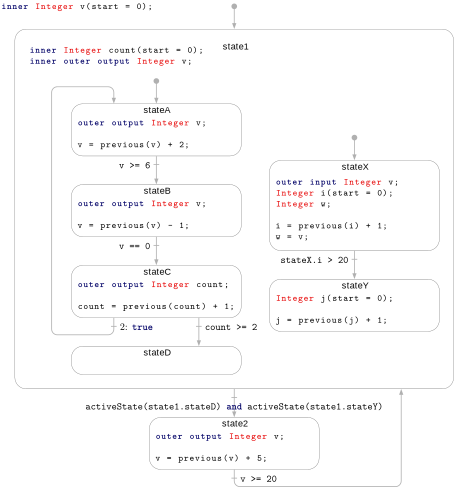
\includegraphics{hierarchical-statemachine}
  \end{center}
  \caption{Example of a hierarchical state machine.}
  \label{fig:hierarchical-statemachine}
\end{figure}

\begin{example}
Consider the hierarchical state machine in \cref{fig:hierarchical-statemachine}.  The model demonstrates the following properties:
\begin{itemize}
\item
  \lstinline!state1! is a meta state with two parallel state machines in it.
\item
  \lstinline!stateA! declares \lstinline!v! as \lstinline!outer output!. \lstinline!state1! is on an intermediate
  level and declares \lstinline!v! as \lstinline!inner outer output!, i.e.\ matches lower level
  \lstinline!outer v! by being \lstinline!inner! and also matches higher level \lstinline!inner v! by being
  \lstinline!outer!. The top level declares \lstinline!v! as \lstinline!inner! and gives the start value.
\item
  \lstinline!count! is defined with a start value in \lstinline!state1!. It is reset when
  a reset transition (\lstinline!v >= 20!) is made to \lstinline!state1!.
\item
  \lstinline!stateX! declares the local variable \lstinline!w! to be equal to \lstinline!v! declared
  as \lstinline!inner input!.
\item
  \lstinline!stateY! declares a local counter \lstinline!j!. It is reset at start and as a
  consequence of the reset transition (\lstinline!v >= 20!) to \lstinline!state1!:
  When the reset transition (\lstinline!v >= 20!) fires, then the variables of the
  active states are reset immediately (so \lstinline!count! from \lstinline!state1!, and \lstinline!i!
  from \lstinline!stateX!). The variables of other states are only reset at the time
  instants when these states become active. So \lstinline!j! in \lstinline!StateY! is reset to
  0, when the transition \lstinline!stateX.i > 20! fires (after \lstinline!state1!
  became active again, so after the reset transition \lstinline!v >= 20!).
\item
  Synchronizing the exit from the two parallel state machines of
  \lstinline!state1! is done by checking that \lstinline!stated! and \lstinline!stateY! are active using the
  \lstinline!activeState! function.
\end{itemize}

The Modelica code (without annotations) is:
\begin{lstlisting}[language=modelica]
block HierarchicalAndParallelStateMachine
  inner Integer v(start=0);

  State1 state1;
  State2 state2;
equation
  initialState(state1);
  transition(state1,state2,activeState(state1.stateD) and
    activeState(state1.stateY), immediate=false);
  transition(state2,state1,v >= 20, immediate=false);

public
  block State1
    inner Integer count(start=0);
    inner outer output Integer v;

    block StateA
      outer output Integer v;
    equation
      v = previous(v) + 2;
    end StateA;
    StateA stateA;

    block StateB
      outer output Integer v;
    equation
      v = previous(v) - 1;
    end StateB;
    StateB stateB;

    block StateC
      outer output Integer count;
    equation
      count = previous(count) + 1;
    end StateC;
    StateC stateC;

    block StateD
    end StateD;
    StateD stateD;

  equation
    initialState(stateA);
    transition(stateA, stateB, v >= 6, immediate=false);
    transition(stateB, stateC, v == 0, immediate=false);
    transition(stateC, stateA, true, immediate=false, priority=2);
    transition(stateC, stateD, count >= 2, immediate=false);

  public
    block StateX
      outer input Integer v;
      Integer i(start=0);
      Integer w; // = v;
    equation
      i = previous(i) + 1;
      w = v;
    end StateX;
    StateX stateX;

    block StateY
      Integer j(start=0);
    equation
      j = previous(j) + 1;
    end StateY;
    StateY stateY;

  equation
    initialState(stateX);
    transition(stateX, stateY, stateX.i > 20, immediate=false,
    reset=false);
  end State1;

  block State2
    outer output Integer v;
  equation
    v = previous(v) + 5;
  end State2;
end HierarchicalAndParallelStateMachine;
\end{lstlisting}

\Cref{fig:state-machine-behavior} shows the behavior of the state machine.
\begin{figure}[H]
  \begin{center}
    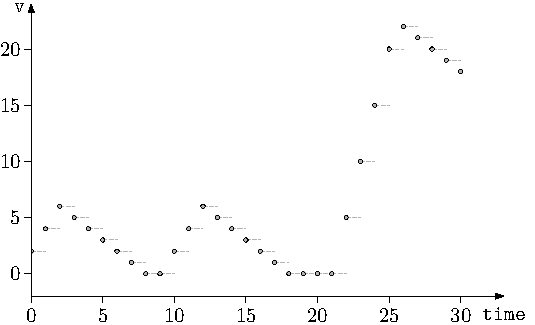
\includegraphics{statemachineplot}
  \end{center}
  \caption{State machine behavior, as reflected by the variable \lstinline!v!.}
  \label{fig:state-machine-behavior}
\end{figure}

The transition from \lstinline!state1! to \lstinline!state2! could have been done with a
\lstinline!synchronize! transition with \lstinline!condition=true! instead. The semantically
equivalent model is shown below:
\begin{lstlisting}[language=modelica]
block HierarchicalAndParallelStateMachine
  extends StateMachineSemantics(
    nStates=2,
    t={Transition(from=1, to=2, immediate=false, synchronize=true),
       Transition(from=2, to=1, immediate=false)},
    c={true, v >= 20});
  Boolean init(start=true) = sample(false);

  block State1
    Boolean active;
    Boolean reset;
    outer input Integer v_previous;
    inner output Integer v;
    inner Integer count(start=0);
    inner Integer count_previous = if reset then 0 else previous(count);

    block StateMachineOf_stateA
      extends StateMachineSemantics(
        nStates=4,
        t={Transition(from=1, to=2, immediate=false),
           Transition(from=2, to=3, immediate=false),
           Transition(from=3, to=1, immediate=false),
           Transition(from=3, to=4, immediate=false)},
        c={v >= 6, v==0, true, count >= 2});
      outer input Integer v_previous;
      outer output Integer v;
      outer input Integer count_previous;
      outer output Integer count;
    equation
      inFinalState = true; // no macro states
      if activeState == 1 then
        // equations for stateA
        v = v_previous + 2;
        count = count_previous;
      elseif activeState == 2 then
        // equations for stateB
        v = v_previous - 1;
        count = count_previous;
      elseif activeState == 3 then
        // equations for stateC
        v = v_previous;
        count = count_previous + 1;
      else // if activeState == 4 then
        // equations for stateD
        v = v_previous;
        count = count_previous;
      end if;
    end StateMachineOf_stateA;

    StateMachineOf_stateA stateMachineOf_stateA(active=active,
      reset=reset);

    block StateMachineOf_stateX
      extends StateMachineSemantics(
        nStates=2,
        t={Transition(from=1, to=2, immediate=false, reset=false)},
        c={i>25});
      outer input Integer v;
      Integer i(start=0);
      Integer i_previous;
      Integer j(start=0);
      Integer j_previous;
      Integer w;
    equation
      inFinalState = true; // no macro states
      if activeState == 1 then
        // equations for stateX
        i_previous = if activeReset or
          activeResetStates[1] then 0 else previous(i);
        j_previous = previous(j);
        i = i_previous + 1;
        w = v;
        j = j_previous;
      else // if activeState == 2 then
        // equations for stateY
        i_previous = previous(i);
        j_previous = if activeReset or activeResetStates[2] then 0 else previous(j);
        i = i_previous;
        w = previous(w);
        j = j_previous + 1;
      end if;
    end StateMachineOf_stateX;

    StateMachineOf_stateX stateMachineOf_stateX(active=active,
      reset=reset);
    Boolean inFinalState = stateMachineOf_stateA.stateMachineInFinalState and
      stateMachineOf_stateX.stateMachineInFinalState;
  end State1;

  State1 state1;
  Integer v(start=0);
  inner Integer v_previous = if reset then 0 else previous(v);
equation
  active = true;
  reset = previous(init);
  if activeState == 1 then
    // equations for state1
    inFinalState = state1.inFinalState;
    state1.active = true;
    state1.reset = activeReset or activeResetStates[1];
    v = state1.v;
  else // if activeState == 2 then
    // equations for state2
    inFinalState = true; // not macro state
    state1.active = false;
    state1.reset = false;
    v = previous(v) + 5;
  end if;
end HierarchcialAndParallelStateMachine;
\end{lstlisting}
\end{example}
